% KSN - wzór sprawozdania
% kodowanie polskich znaków: ISO-8859-2

\documentclass[10pt,a4paper]{article}
\usepackage[margin=2cm]{geometry}
\usepackage{graphicx}
\usepackage[utf8]{inputenc}
\usepackage[polish]{babel}
\usepackage{polski}
\usepackage{amsmath}
\usepackage{mathtools}
\usepackage{subcaption}
\usepackage{float}
\author{Ryniak}

\begin{document}

% =====  STRONA TYTULOWA PRACY INŻYNIERSKIEJ ====
% ostatnia modyfikacja: 2011/03/09, K. Malarz

\thispagestyle{empty}
\vspace*{50ex}
\begin{center}
{\bf\LARGE\textsf{Sprawozdanie do projeku:}}\\
\vspace{5ex}

{\bf\huge\textsf{Wykorzystanie probabilistycznych sieci neuronowych do klasyfikacji danych o zmiennym charakterze}}\\
\vspace{54ex}

{\bf\Large\textsf{Grzegorz Ryniak, Rafał Szęszoł}}\\
\vspace{22ex}
\textsf{\bf\large\textsf{Kraków, czerwiec 2018}}
\end{center}


\newpage

\section{Wstęp}
W świecie rzeczywistym często spotykamy się ze źródłami informacji, które z czasem zaczynają przesyłać zmodyfikowane dane. Przykładem może być elektroniczny czujnik grubości - odpowiednik czujnika zegarkowego. W skutek zużycia np. końcówek pomiarowych, z czasem otrzymywane wartości mogą być zaniżone. Duży problem pojawia się kiedy odbierane dane poddawane są klasyfikacji. Klasyfikator widząc przesunięcie danych może uznać, że należą one do innej klasy. Z czasem tych klas mogło by powstać coraz więcej. Ze względu na ograniczone zasoby i łatwość interpretacji często wymaga się, aby liczba klas była stała. Celem tego projektu było stworzenie klasyfikatora opartego o probabilistyczne sieci neuronowe, który byłby w stanie na bieżąco dostosowywać się do zmiennych danych. 

\section{Doświadczenia}
Wszystkie symulacje zostały przeprowadzone z wykorzystaniem środowiska MATLAB 2012b. W pierwszej kolejności stworzono generator danych, który symulował by rzeczywiste źródło informacji podlegające zużyciu. Stworzone zostały 2 zestawy danych. Generowane były po 2 klasy dwu-wymiarowych danych. Dane takie łatwo da się przedstawić na układzie współrzędnych w postaci punktów. W pierwszym zestawie pierwsza klasa składała się z punktów o współrzędnych generowanych z rozkładu Gaussa o średniej wartości (0;0) i odchyleniu 1, natomiast druga klasa również była generowana na podstawie rozkładu Gaussa o średnim odchyleniu 1 ale średnie wartości były punktami leżącymi na okręgu o promieniu 2 i środku w punkcie (0;0). Kąt pomiędzy osią x a promieniem zwiększał się z czasem w kierunku przeciwnym do wskazówek zegara. Co 90 stopni ruch na chwilę się zatrzymywał, aby sprawdzić, czy sieć nie przyzwyczaiła się do ruchu. Generowanie danych kończy się w momencie kiedy druga klasa ,,okrąży'' pierwszą dookoła. Kolejne etapy generowania danych pokazane są na rysunku \ref{dataGen}. 
\begin{figure}[H]
  \begin{subfigure}[b]{0.4\textwidth}
    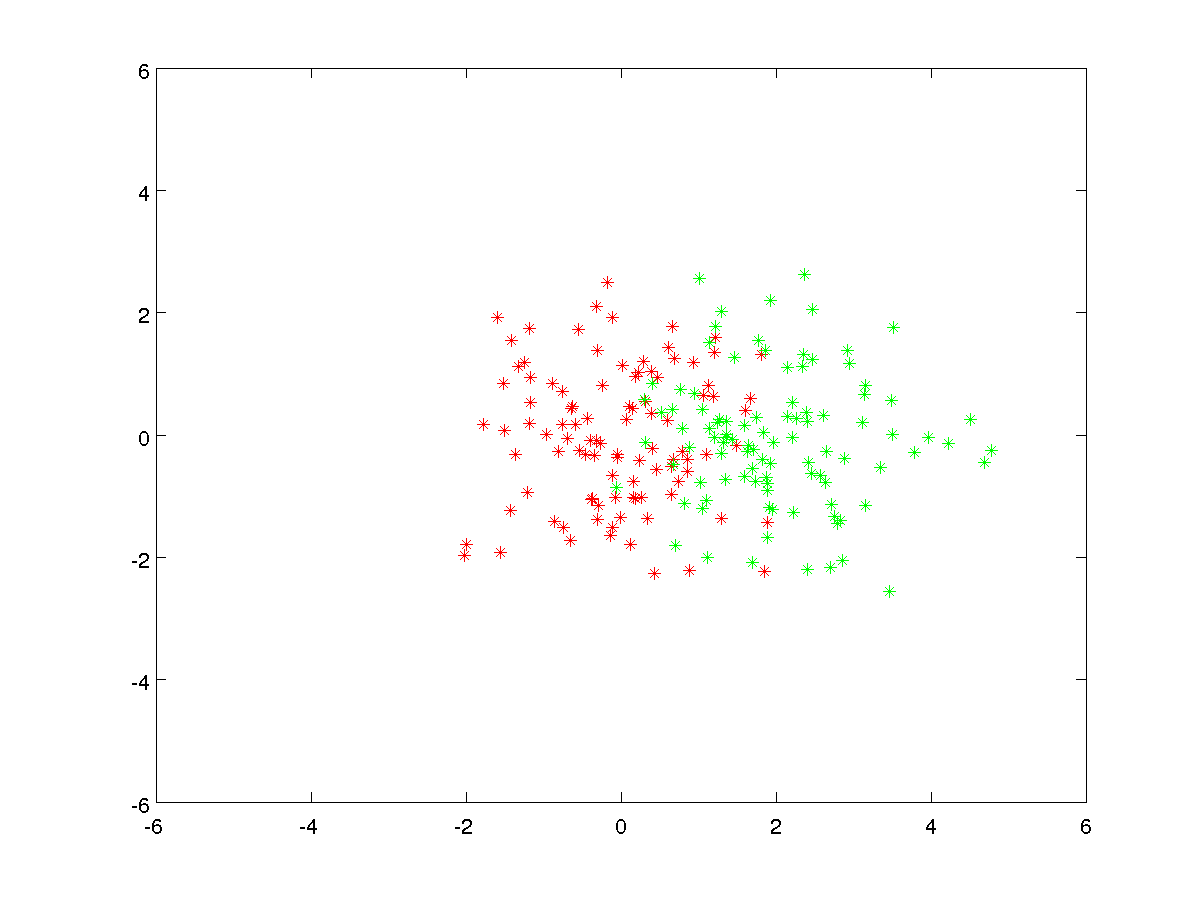
\includegraphics[width=\textwidth]{dataGen_step0.png}
    \caption{Krok 1}
  \end{subfigure}
  \hfill
  \begin{subfigure}[b]{0.4\textwidth}
    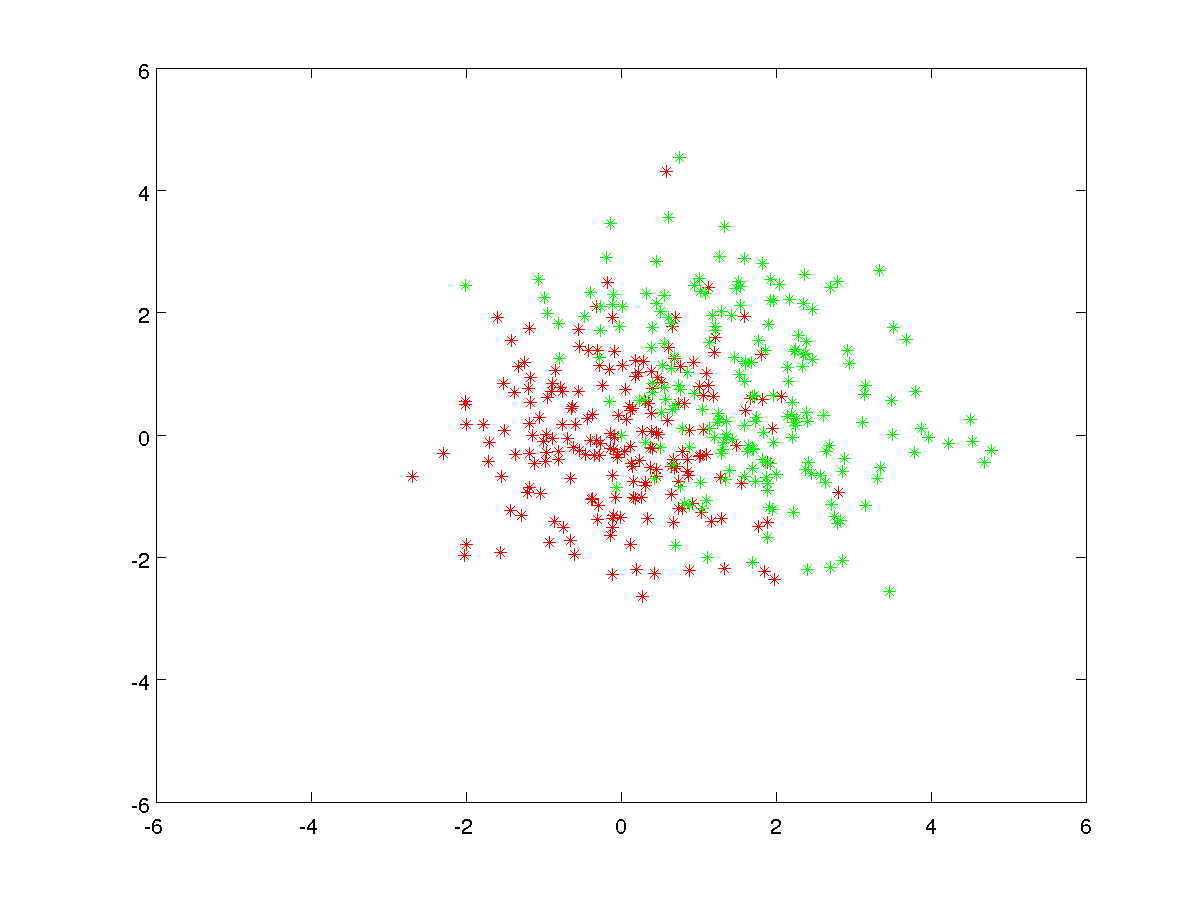
\includegraphics[width=\textwidth]{dataGen_step1.png}
    \caption{Krok 2}
  \end{subfigure}

   \begin{subfigure}[b]{0.4\textwidth}
    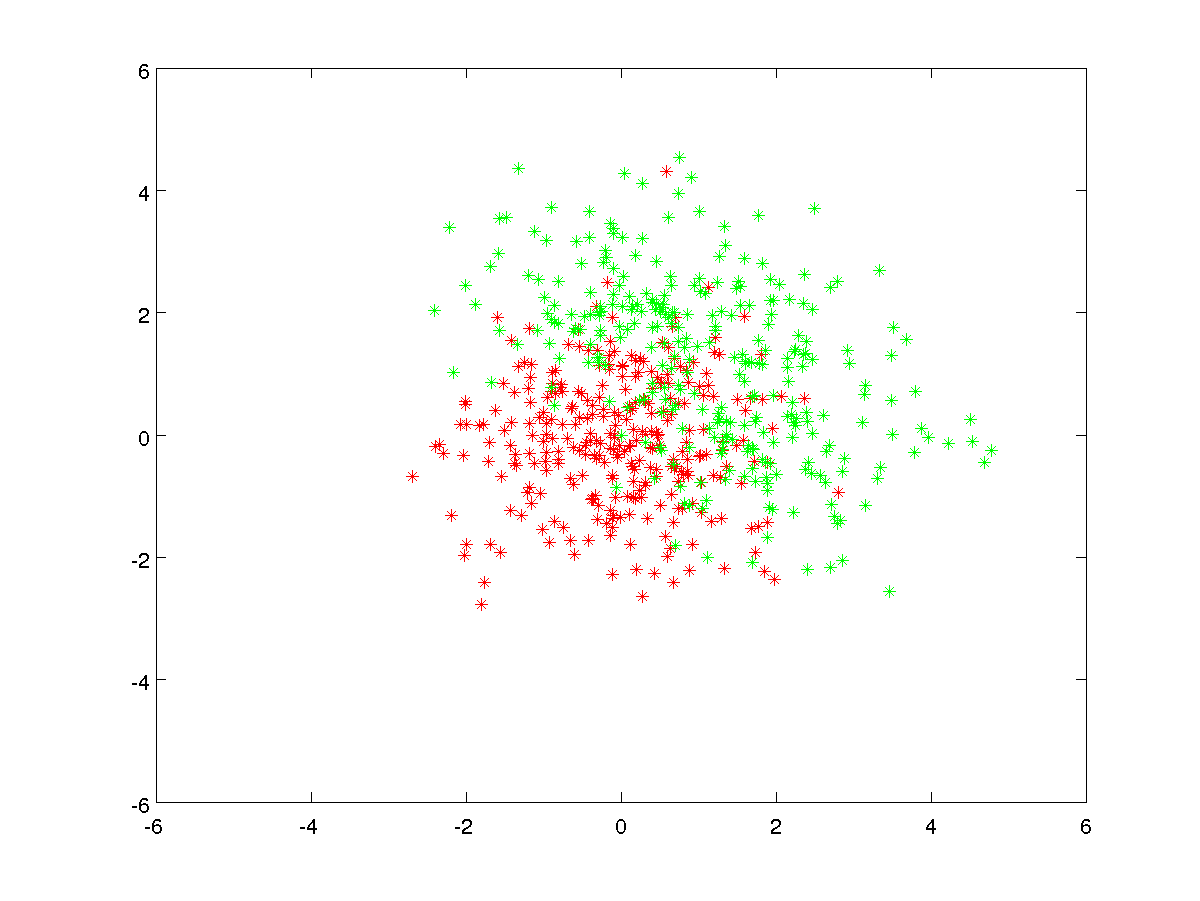
\includegraphics[width=\textwidth]{dataGen_step2.png}
    \caption{Krok 3}
  \end{subfigure}
  \hfill
  \begin{subfigure}[b]{0.4\textwidth}
    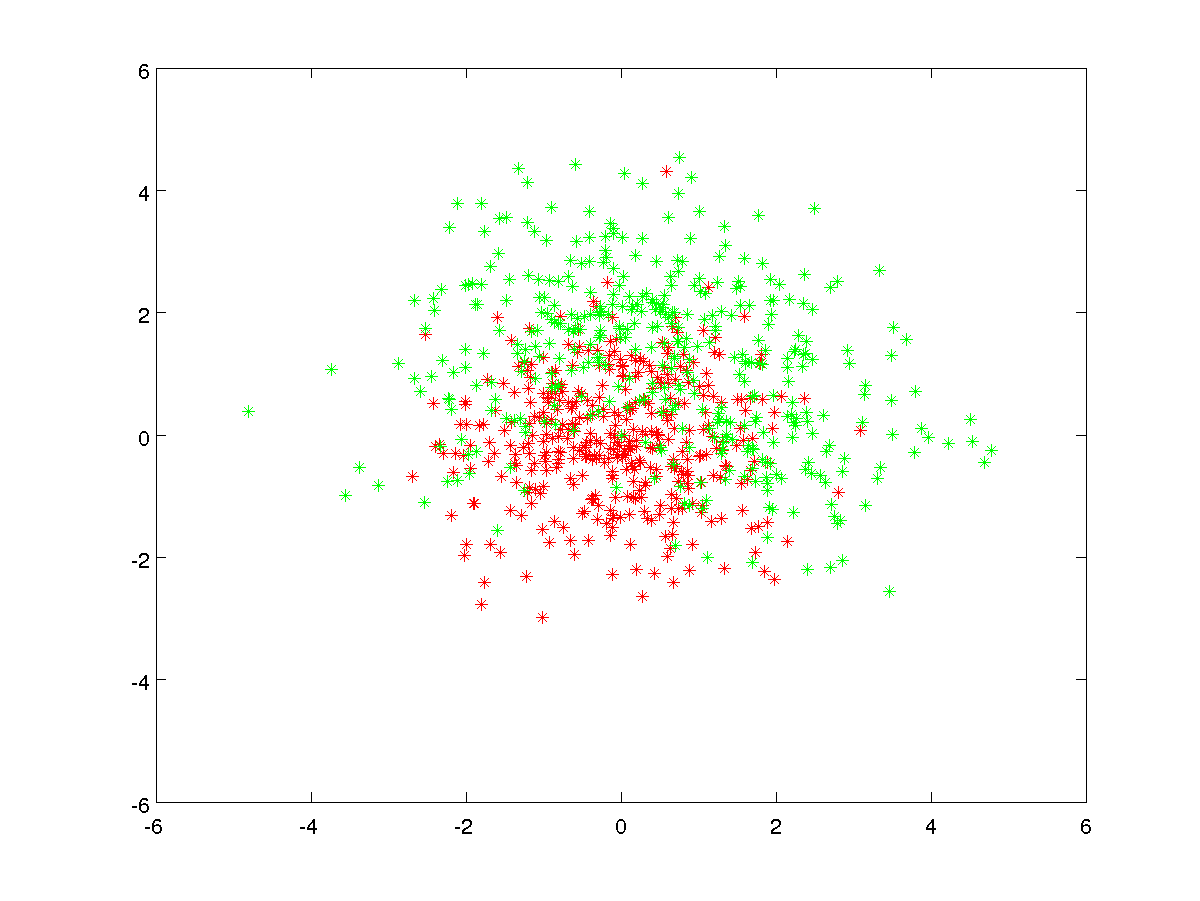
\includegraphics[width=\textwidth]{dataGen_step3.png}
    \caption{Krok 4}
  \end{subfigure}
  
  \begin{subfigure}[b]{0.4\textwidth}
    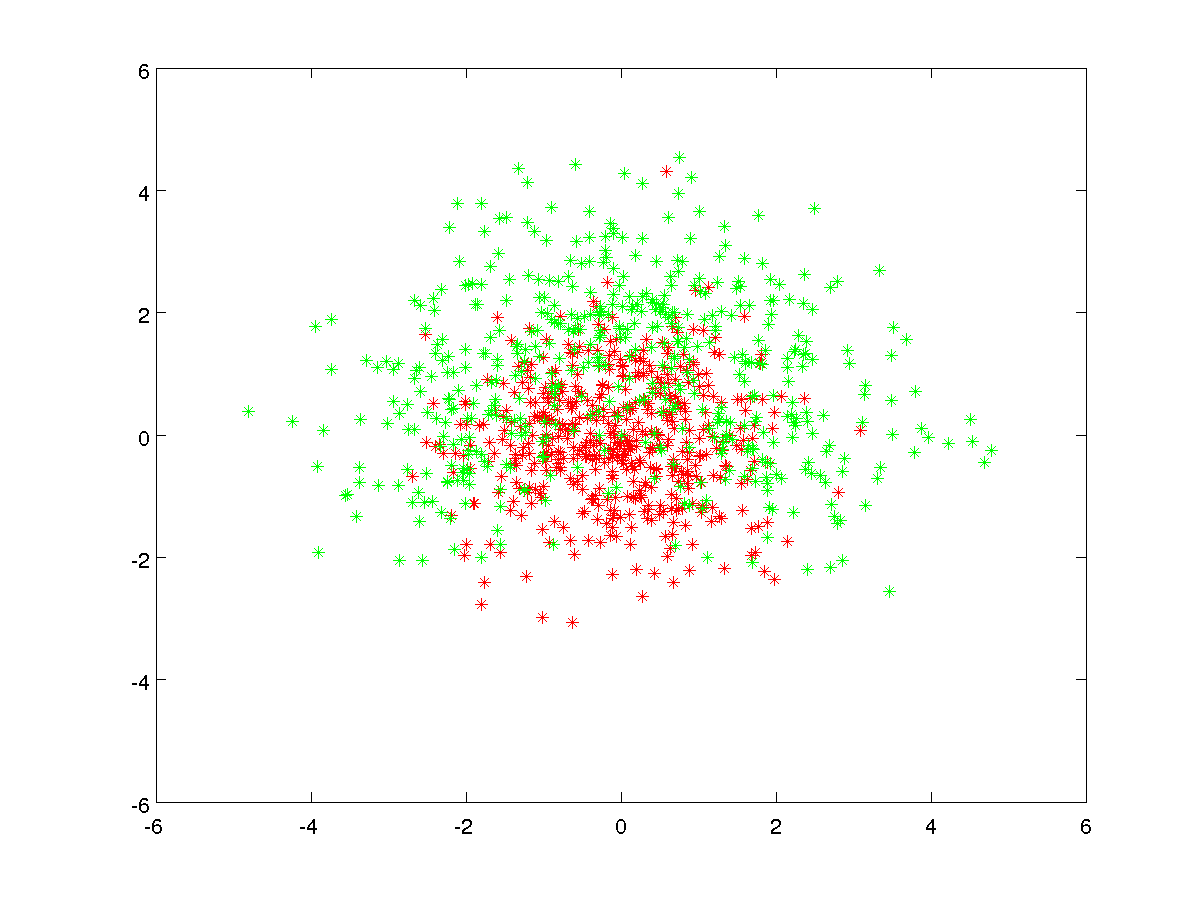
\includegraphics[width=\textwidth]{dataGen_step4.png}
    \caption{Krok 5}
  \end{subfigure}
  \hfill
  \begin{subfigure}[b]{0.4\textwidth}
    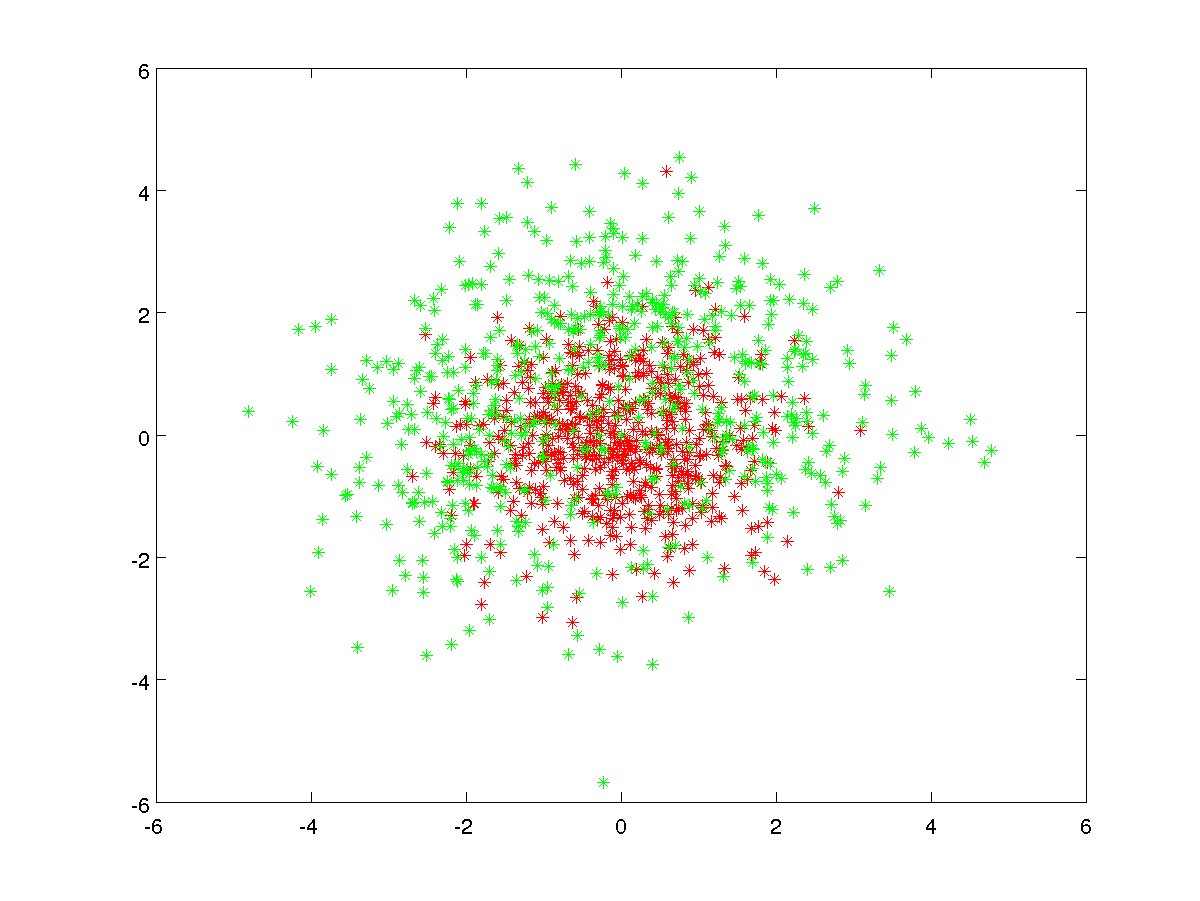
\includegraphics[width=\textwidth]{dataGen_step5.png}
    \caption{Krok 6}
  \end{subfigure}
  
  \begin{center}
  \begin{subfigure}[b]{0.4\textwidth}
    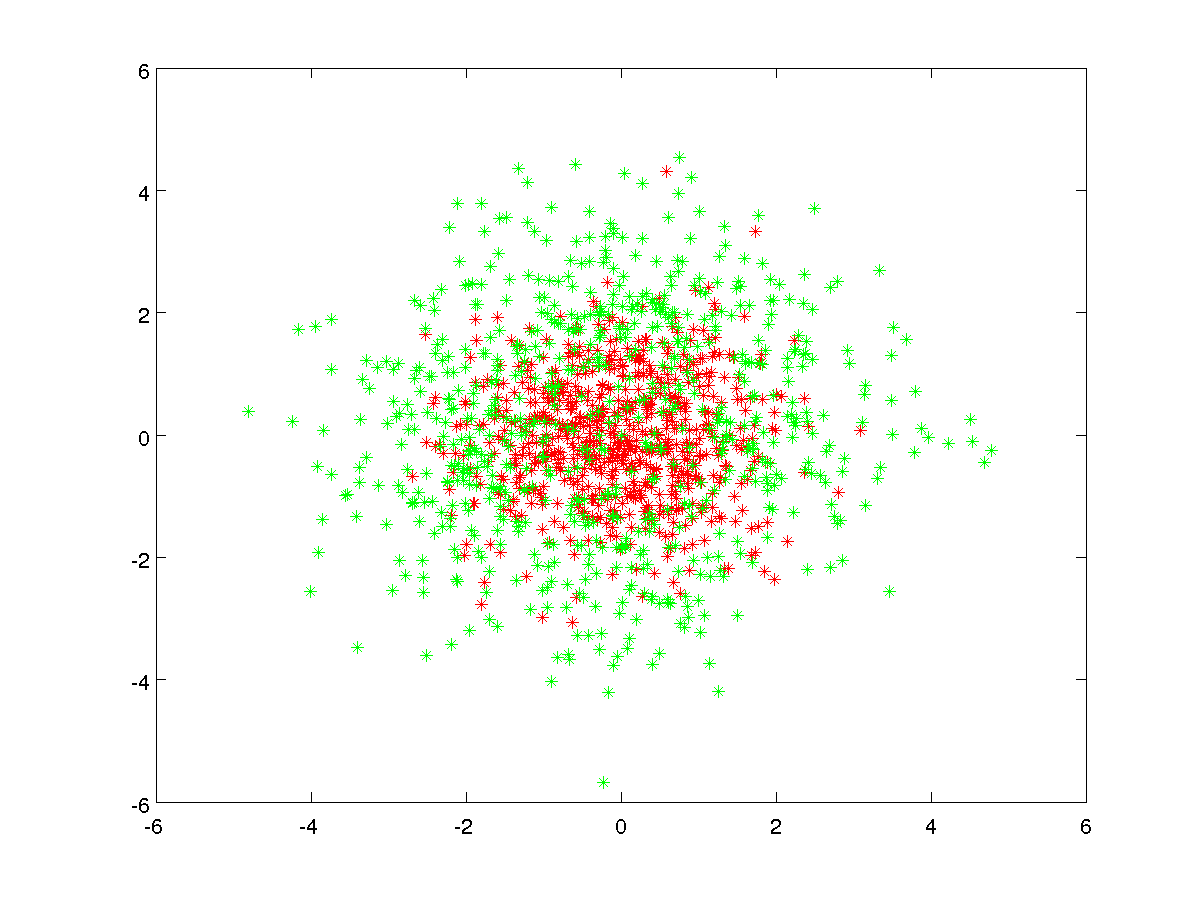
\includegraphics[width=\textwidth]{dataGen_step6.png}
    \caption{Krok 7}
  \end{subfigure}
  \end{center}
  
  \caption{Poszczególne etapy generowania danych dla zestawu pierwszego}
  \label{dataGen}
  
\end{figure}

Drugi zestaw składał się również z dwóch dwu wymiarowych klas. Pierwsza klasa składała się z punktów rozsianych wg rozkładu Gaussa z dwoma punktami centralnymi (-2,0) i (2,0). Druga klasa przemieszczała się po "ósemce" - dwóch połączonych okręgach wokół klasy pierwszej. Promień okręgu wynosił 4. Odchylenie standardowe przy rozkładzie Gaussa w obu klasach wyniosło 1. Kolejne etapy generowania danych dla zestawy 2 pokazane są na rysunku \ref{dataGen2}. 

\ref{dataGen}. 
\begin{figure}[H]
  \begin{subfigure}[b]{0.4\textwidth}
    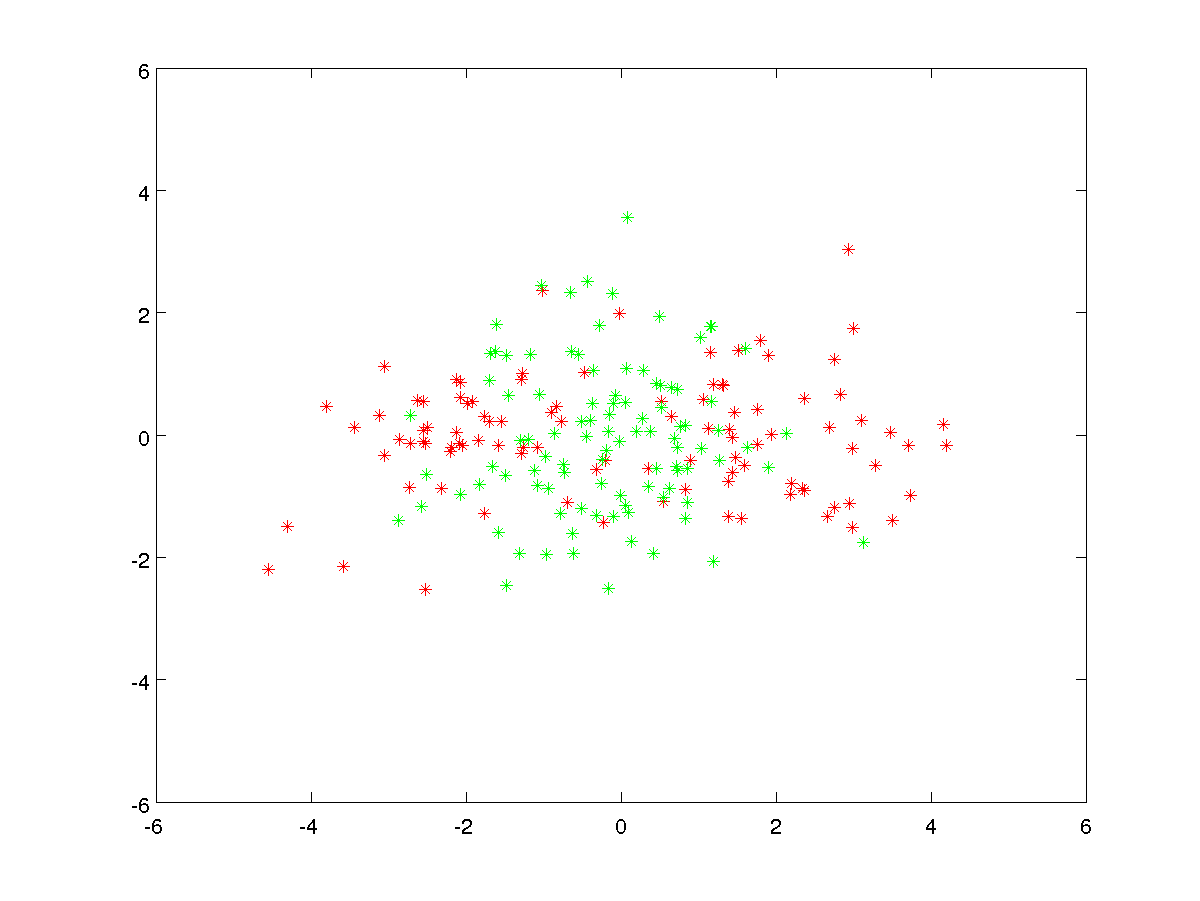
\includegraphics[width=\textwidth]{dataGen2_step0.png}
    \caption{Krok 1}
  \end{subfigure}
  \hfill
  \begin{subfigure}[b]{0.4\textwidth}
    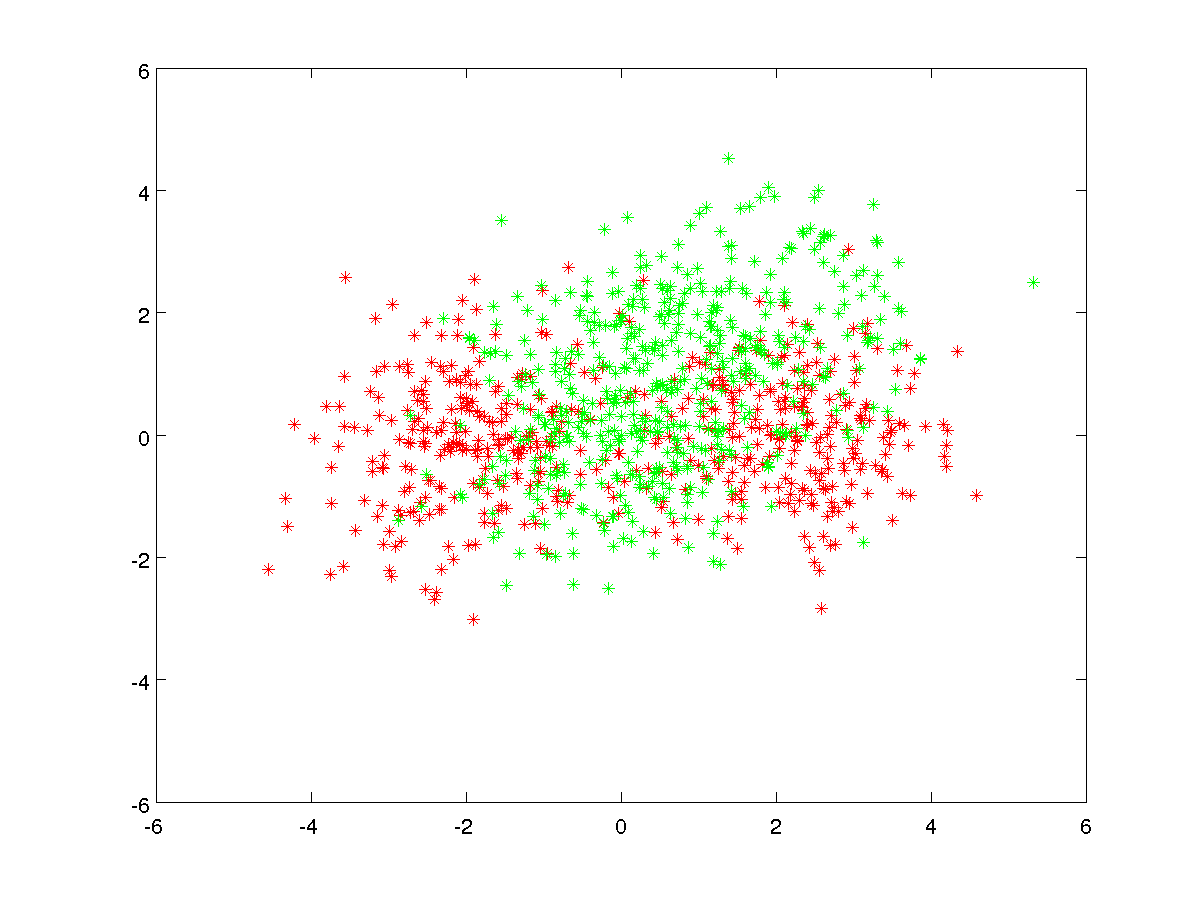
\includegraphics[width=\textwidth]{dataGen2_step1.png}
    \caption{Krok 2}
  \end{subfigure}

   \begin{subfigure}[b]{0.4\textwidth}
    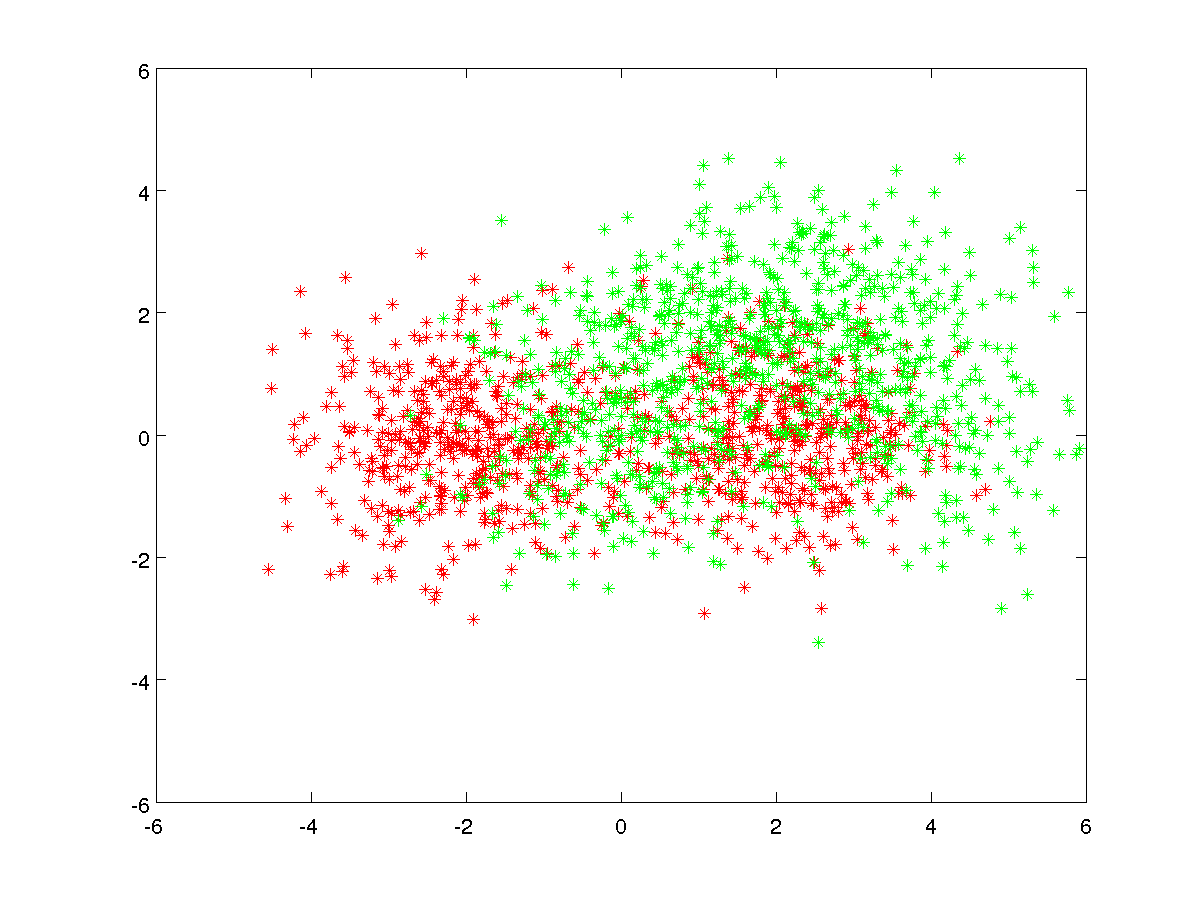
\includegraphics[width=\textwidth]{dataGen2_step2.png}
    \caption{Krok 3}
  \end{subfigure}
  \hfill
  \begin{subfigure}[b]{0.4\textwidth}
    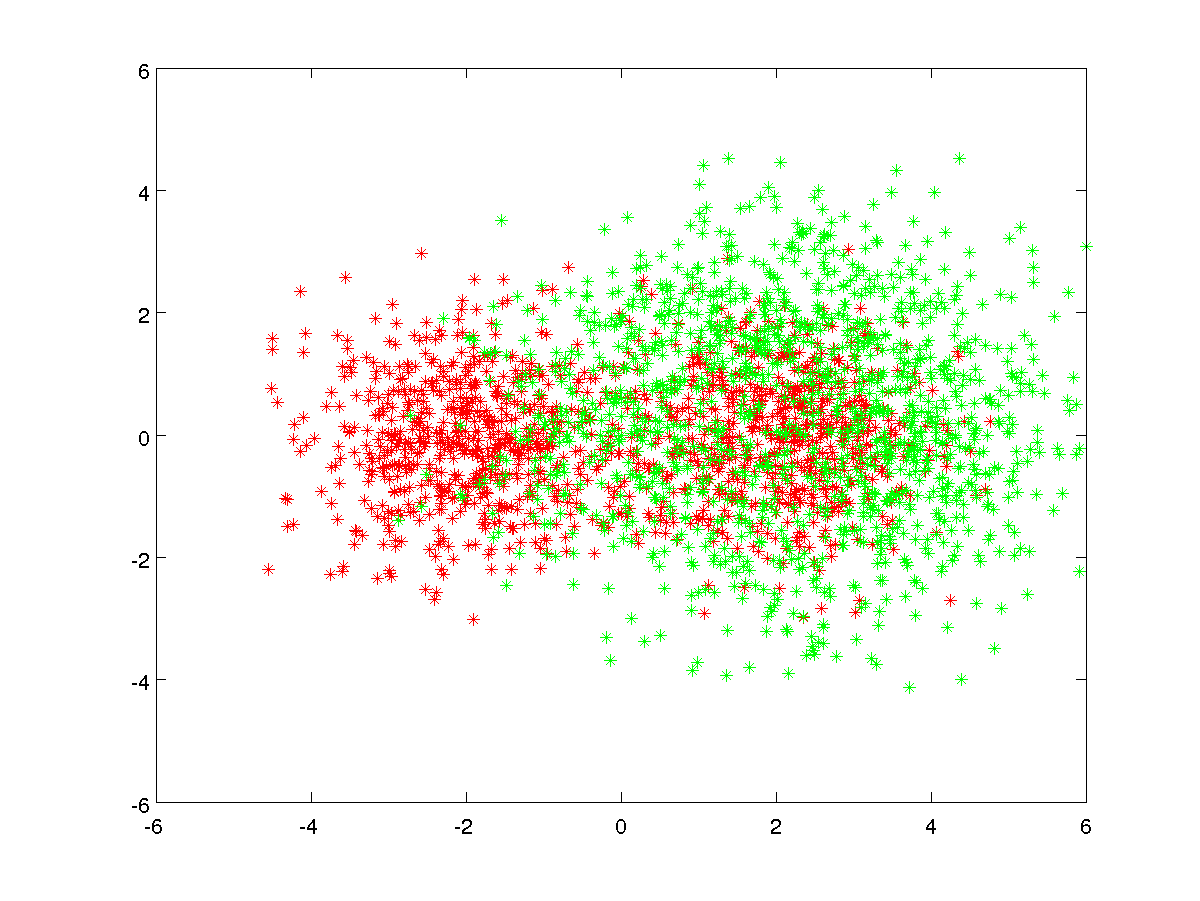
\includegraphics[width=\textwidth]{dataGen2_step3.png}
    \caption{Krok 4}
  \end{subfigure}
  
  \begin{subfigure}[b]{0.4\textwidth}
    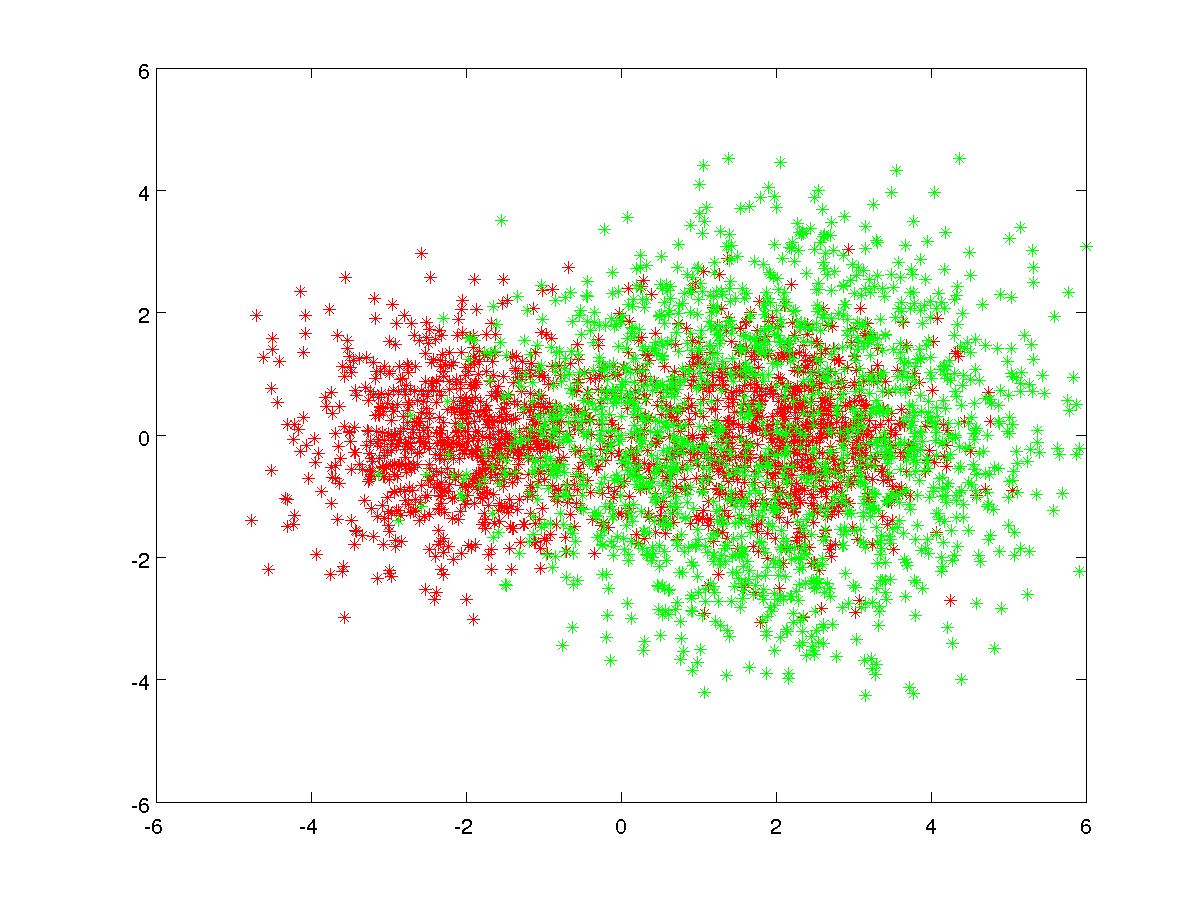
\includegraphics[width=\textwidth]{dataGen2_step4.png}
    \caption{Krok 5}
  \end{subfigure}
  \hfill
  \begin{subfigure}[b]{0.4\textwidth}
    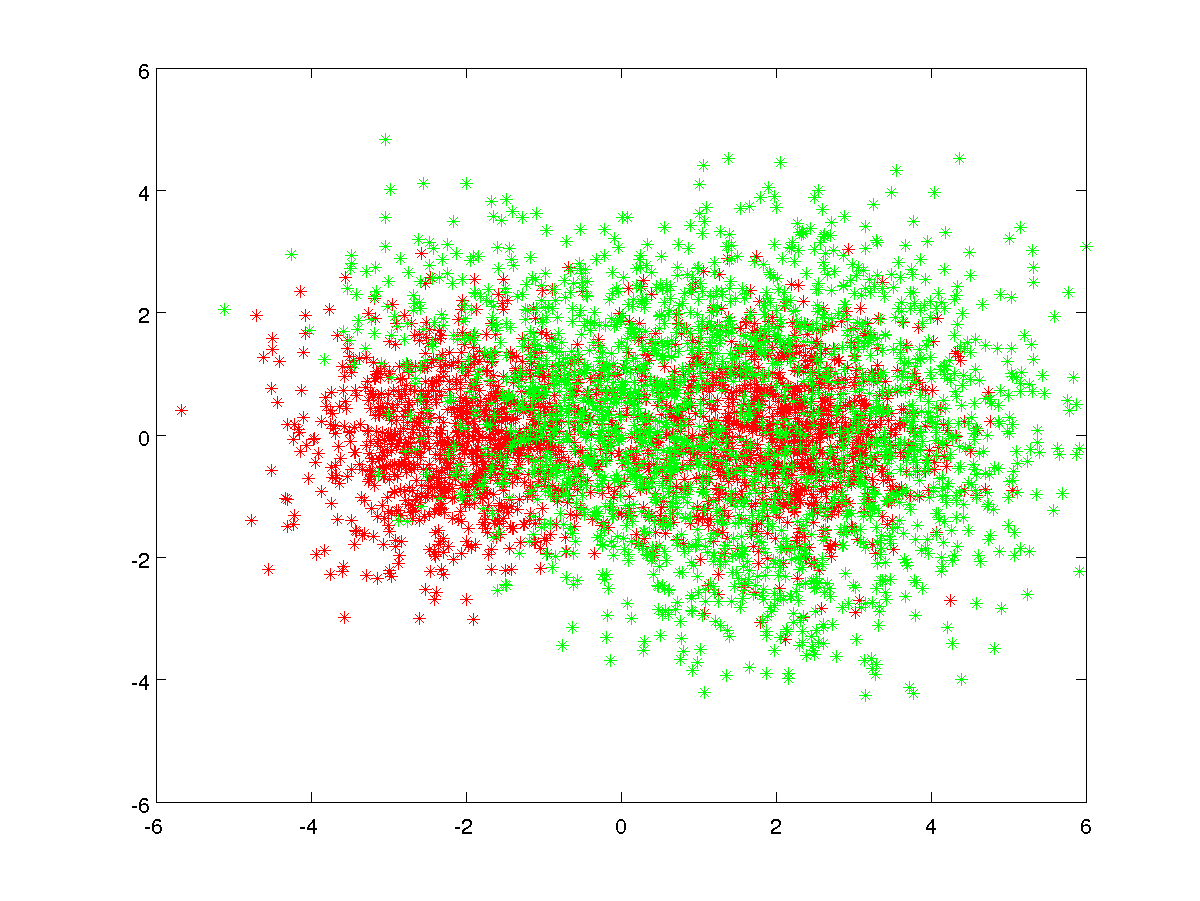
\includegraphics[width=\textwidth]{dataGen2_step5.png}
    \caption{Krok 6}
  \end{subfigure}
  
   \begin{subfigure}[b]{0.4\textwidth}
    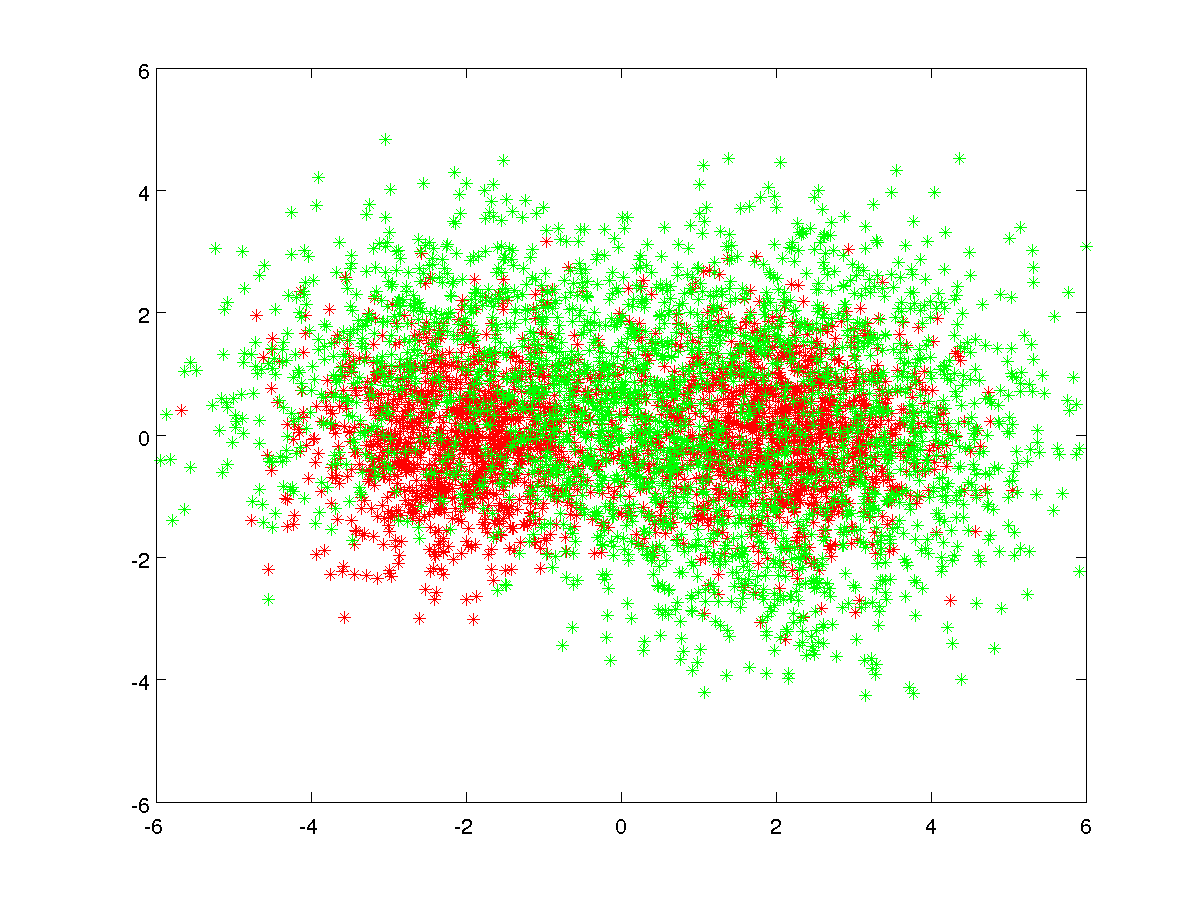
\includegraphics[width=\textwidth]{dataGen2_step6.png}
    \caption{Krok 7}
  \end{subfigure}
  \hfill
  \begin{subfigure}[b]{0.4\textwidth}
    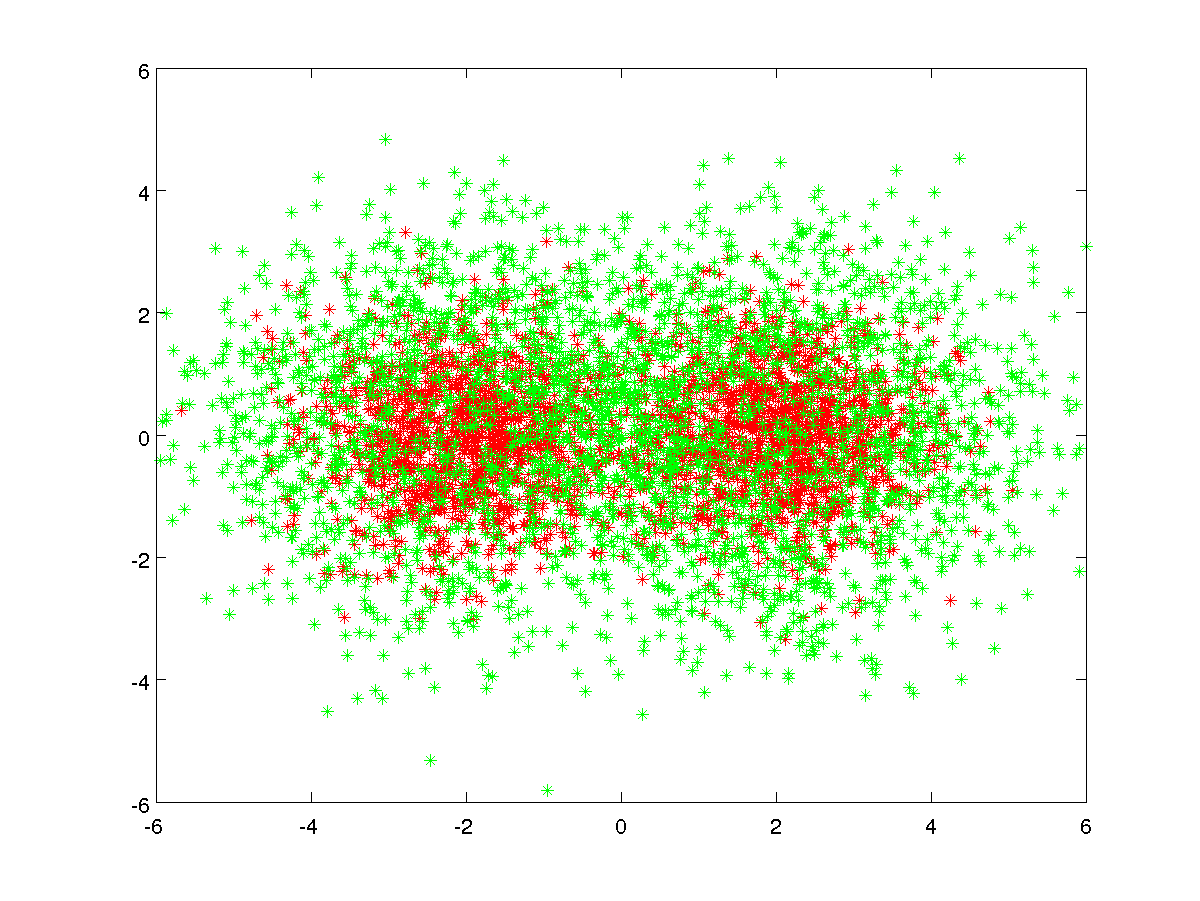
\includegraphics[width=\textwidth]{dataGen2_step7.png}
    \caption{Krok 8}
  \end{subfigure}
  
  \caption{Poszczególne etapy generowania danych dla zestawu drugiego}
  \label{dataGen2}
  
\end{figure}

Liczbę punktów generowanych w każdym kroku można było zmieniać. Co określoną ilość dodanych punktów sieć neuronowa była uczona nowych danych. Podczas ponownego uczenia sieci, zmianom podlegał parametr wygładzania. Algorytm wyznaczania tegoż parametru został dostarczony przez prowadzącego zajęcia. Podczas symulacji wykonywany był wykres jak w czasie zmienia się procent błędnie sklasyfikowanych punktów oraz mapa, gdzie te punkty się znajdowały. Wartość błędu była ułamkiem wyrażonym w procentach oznaczającym ilość błędnych klasyfikacji w obrębie całego okna na ilość dodanych nowych punktów, zatem wartość ta może przekroczyć 100 \%. 

\subsection{Metoda stałego okna}
W metodzie kolejkowej dane, na których uczyła się sieć znajdowały się w kolejce. Kiedy do kolejki wchodził nowy punkt, najstarszy zostawał z niej usuwany. Długość kolejki mogła być regulowana. 

Na początku przeprowadzono testy dla stałego parametru wygładzania (wartość spread) na zestawie pierwszym. Liczbę wszystkich generowanych punktów ustawiono na 9000. Rozmiar okna wynosił 200 punktów. Symulacje przeprowadzono dla spread równego 0,001; 0,01; 0,1; 1, 10 oraz 15. Dla każdego testu sporządzona został mapa z błędnymi punktami w ostatniej fazie, wykres zależności błędu od czasu oraz średnia wartość błędu. Wyniki przedstawia rysunek \ref{test_h} oraz tabela \ref{h_table}.

\begin{figure}[H]

   \begin{subfigure}[b]{0.5\textwidth}
    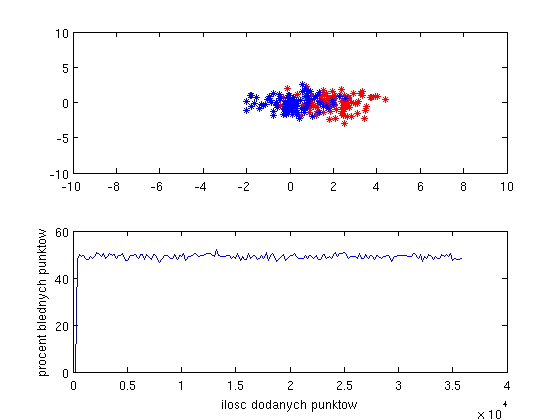
\includegraphics[width=\textwidth]{test_h0_001.png}
    \caption{h = 0,001}
  \end{subfigure}
  \hfill
  \begin{subfigure}[b]{0.5\textwidth}
    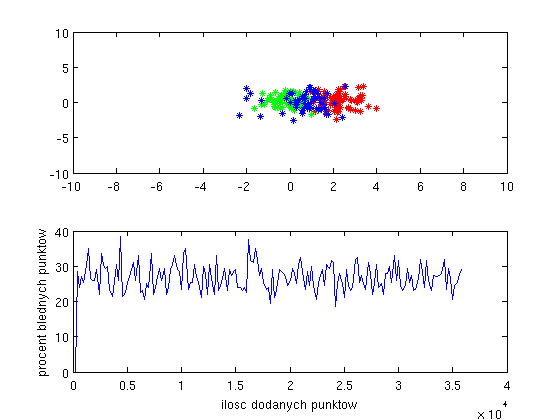
\includegraphics[width=\textwidth]{test_h0_01.png}
    \caption{h = 0,01}
  \end{subfigure}
  
   \begin{subfigure}[b]{0.5\textwidth}
    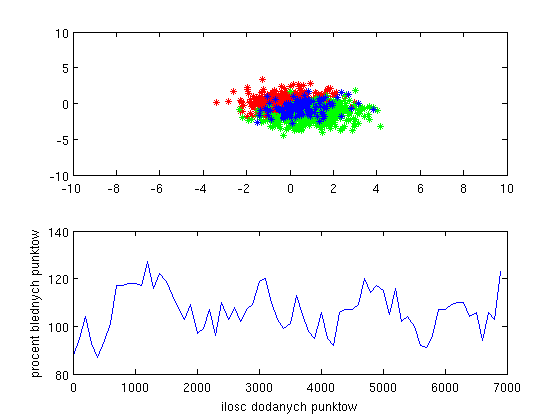
\includegraphics[width=\textwidth]{test_h0_1.png}
    \caption{h = 0,1}
  \end{subfigure}
  \hfill
  \begin{subfigure}[b]{0.5\textwidth}
    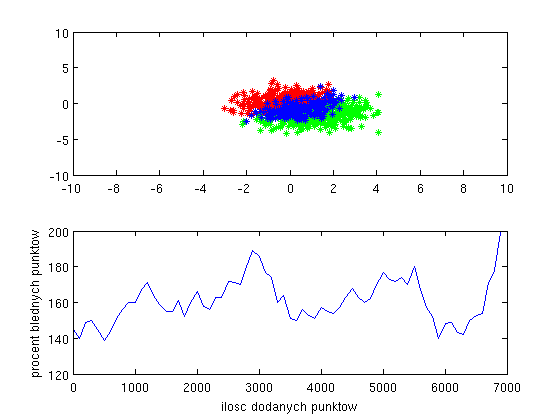
\includegraphics[width=\textwidth]{test_h1.png}
    \caption{h = 1}
  \end{subfigure}
  
     \begin{subfigure}[b]{0.5\textwidth}
    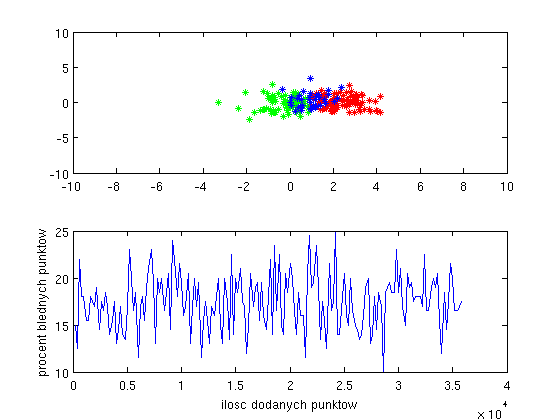
\includegraphics[width=\textwidth]{test_h10.png}
    \caption{h = 10}
  \end{subfigure}
  \hfill
  \begin{subfigure}[b]{0.5\textwidth}
    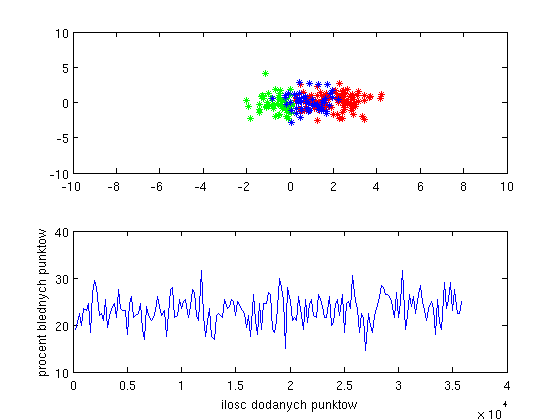
\includegraphics[width=\textwidth]{test_h15.png}
    \caption{h = 15}
  \end{subfigure}
  
  \caption{Test zestawu 1 dla różnych h}
  \label{test_h}
  
\end{figure}



\begin{table}[H]
\centering
\begin{tabular}{|c|c|}
\hline
spread & błąd \\
\hline
0,001 & 48\%  \\
\hline
0,01 & 26\%  \\
\hline
0,1 & 22\%  \\
\hline
1 & 16\%  \\
\hline
10 & 18\%  \\
\hline
15 & 23\%  \\
\hline
\end{tabular}
\caption{Zestawienie wyników testów dla stałych wartości spread dla zestawu 1.}
\label{h_table}
\end{table}


Następnie przeprowadzono symulację dla h - wartości spread liczonej automatycznie. 

Parametry danych były jak w poprzednim przypadku. Rysunek \ref{test_h_auto} przedstawia otrzymane wyniki. Sporządzone wyniki zostały uzupełnione o wartość współczynnika wygładzenia zmieniającego się w czasie. 

\begin{figure}[H]
\centering
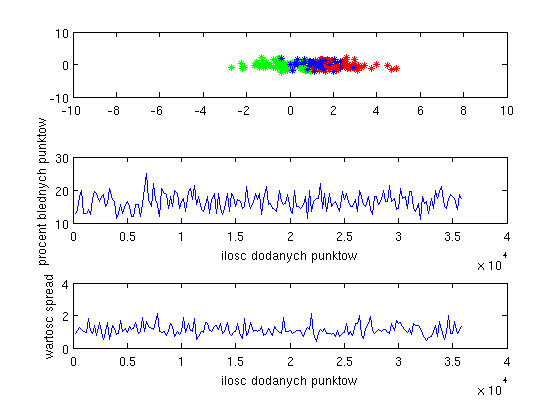
\includegraphics[width=15cm]{test_h_auto_16_47.png}
\caption{Symulacja dla spread liczonego automatycznie.}
\label{poj}
\end{figure}

Średni błąd wyniósł 40 \%. 

%zestaw 2

Analogiczny test został przeprowadzony dla zestawu nr 2. 
Wyniki przedstawia rysunek \ref{test_h2} oraz tabela \ref{h_table2}.

\begin{figure}[H]

   \begin{subfigure}[b]{0.5\textwidth}
    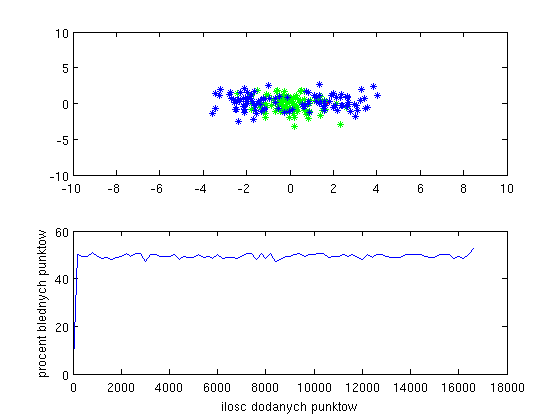
\includegraphics[width=\textwidth]{test2_h0_001.png}
    \caption{h = 0,001}
  \end{subfigure}
  \hfill
  \begin{subfigure}[b]{0.5\textwidth}
    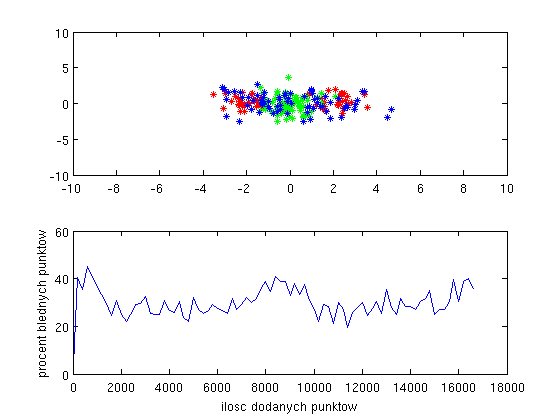
\includegraphics[width=\textwidth]{test2_h0_01.png}
    \caption{h = 0,01}
  \end{subfigure}
  
   \begin{subfigure}[b]{0.5\textwidth}
    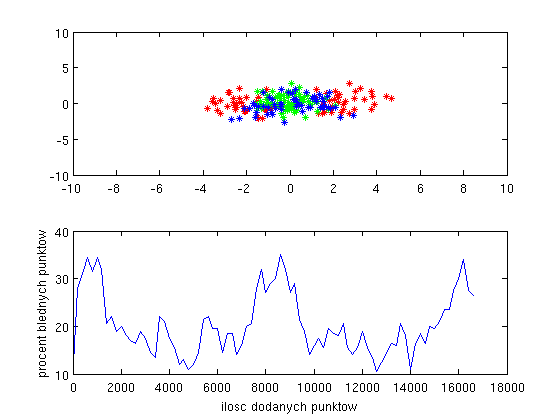
\includegraphics[width=\textwidth]{test2_h0_1.png}
    \caption{h = 0,1}
  \end{subfigure}
  \hfill
  \begin{subfigure}[b]{0.5\textwidth}
    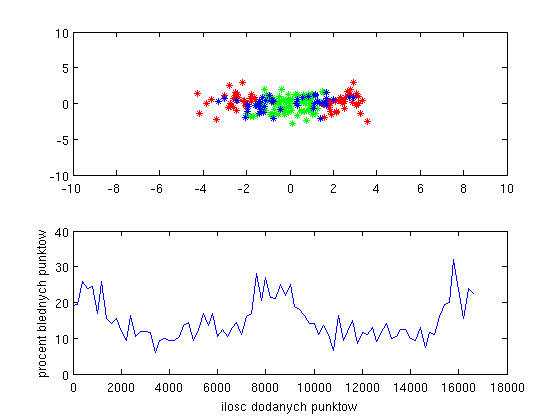
\includegraphics[width=\textwidth]{test2_h1.png}
    \caption{h = 1}
  \end{subfigure}
  
     \begin{subfigure}[b]{0.5\textwidth}
    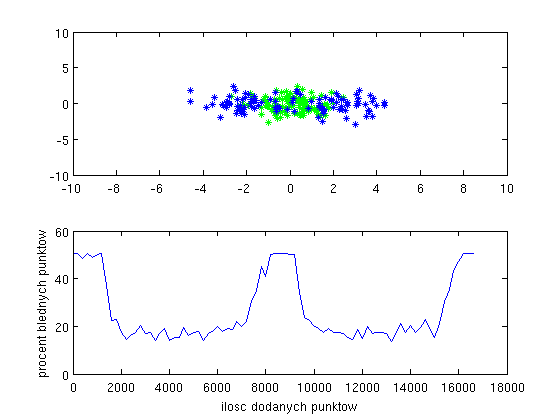
\includegraphics[width=\textwidth]{test2_h10.png}
    \caption{h = 10}
  \end{subfigure}
  \hfill
  \begin{subfigure}[b]{0.5\textwidth}
    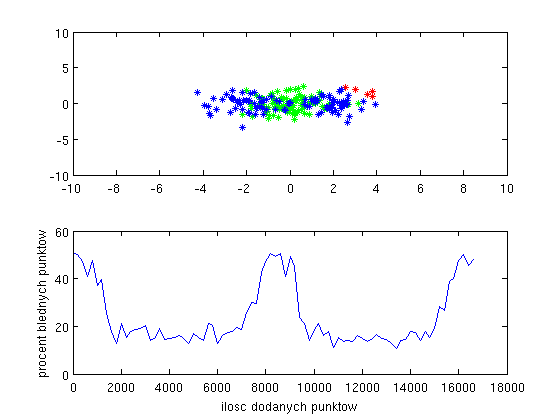
\includegraphics[width=\textwidth]{test2_h15.png}
    \caption{h = 15}
  \end{subfigure}
  
  \caption{Test zestawu 2 dla różnych h}
  \label{test_h2}
  
\end{figure}



\begin{table}[H]
\centering
\begin{tabular}{|c|c|}
\hline
spread & błąd \\
\hline
0,001 & 48\%  \\
\hline
0,01 & 29\%  \\
\hline
0,1 & 20\%  \\
\hline
1 & 15\%  \\
\hline
10 & 26\%  \\
\hline
15 & 23\%  \\
\hline
\end{tabular}
\caption{Zestawienie wyników testów dla stałych wartości spread dla zestawu 2.}
\label{h_table2}
\end{table}

%%----------------------------METODA_PRIORYTETÓW
\subsection{Metoda priorytetów}
Analogiczne testy przeprowadzono dla metody priorytetowej. Polegała ona na tym, że punkty służące do uczenia sieci w kolejnych krokach były trzymane w buforze o stałej wielkości. Kiedy przychodził nowy punkt, liczony był jego priorytet na podstawie prawdopodobieństwa przynależności do danej klasy oraz jego wieku. Dla punktów w buforze aktualizowano wartość priorytetu, ponieważ punkty w buforze się starzały. Nowy punkt był dodawany do bufora. Następnie odbywało się sortowanie wg priorytetu i usuwany był punkt z najniższą jego wartością. Priorytet punktów był liczony głównie w funkcji \textit{comptScore} oraz jego przyczynki częściowo w innych częściach programu, według następującego wzoru:
\begin{gather}
	\alpha(x_{i}^{(g)}) = \frac{t_{max} - t(x_i)}{2t_{max}} + \eta y^{(g)}(x_i) - \gamma \Bigg( \sum_{k=1}^K\Big(y^{(k)}(x_i)\Big) -y^{(g)}(x_i) \Bigg),
\end{gather}
gdzie $\alpha(x_{i}^{(g)})$ oznacza priorytet i-tego punktu z klasy g, $t_{max}$ maksymalny wiek punktu (powyżej maksymalnego wieku, punkt zaczyna otrzymywać karę za wiek), $t(x_i)$ - wiek  punktu, K - liczba klas, $y^{(k)}$ prawdopodobienstwo przynaleznosci do k-tej klasy, $\eta$ oraz $\gamma$ - współczynniki. W powyższym wzorze $y^{(g)}(x)$ liczone jest jako:


\begin{gather}
	y^{(g)}(x) = \frac{1}{l_g(2\pi)^{n/2}\sigma^n}  \sum_{j=1}^{l_g}exp\Bigg(-\sum_{j=1}^n\frac{(x_{ij}^{(g)} - x_j)^2}{2\sigma^2} \Bigg),
\end{gather}
gdzie $l_g$ oznacza liczbę punktów klasy g, $n$ liczbę atrybutów klasy (w przypadku punktów współrzędne x i y), $\sigma$ parametr $spread$, $x_{ij}^{(g)}$ oznacza j-ty atrybut i-tej punktu z klasy g. 
Dla obu zestawów przeprowadzono symulacje dla h równego 0,001, 0,01; 0,1; 1, 10 i 100. W drugim zestawie wprowadzono modyfikację polegającą na rozbiciu klasy stacjonarnej na dwie klasy (o centrach w pkt. (-2,0) i (2,0). Szerokość okna wynosiła 50. Wyniki dla zestawu pierwszego przedstawia rysunek \ref{test_h3} oraz tabela \ref{h_table3}.

\begin{figure}[H]

   \begin{subfigure}[b]{0.5\textwidth}
    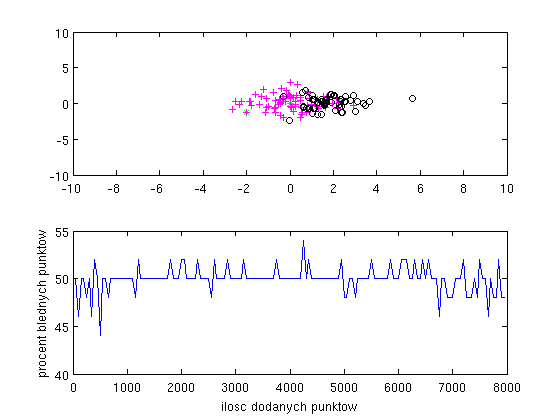
\includegraphics[width=\textwidth]{test3_h0_001_50_00.png}
    \caption{h = 0,001}
  \end{subfigure}
  \hfill
  \begin{subfigure}[b]{0.5\textwidth}
    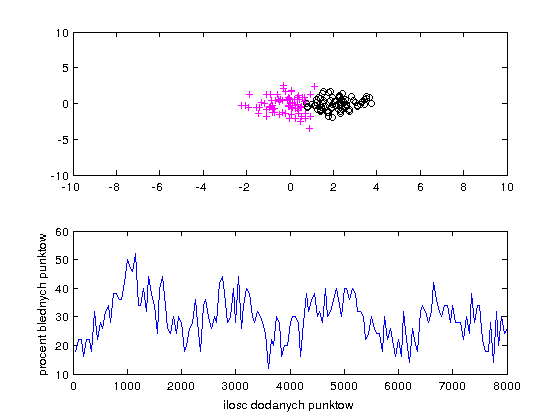
\includegraphics[width=\textwidth]{test3_h0_01_29_7.png}
    \caption{h = 0,01}
  \end{subfigure}
  
   \begin{subfigure}[b]{0.5\textwidth}
    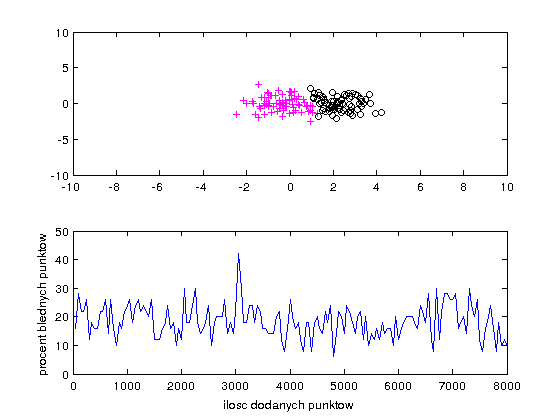
\includegraphics[width=\textwidth]{test3_h0_1_18_5.png}
    \caption{h = 0,1}
  \end{subfigure}
  \hfill
  \begin{subfigure}[b]{0.5\textwidth}
    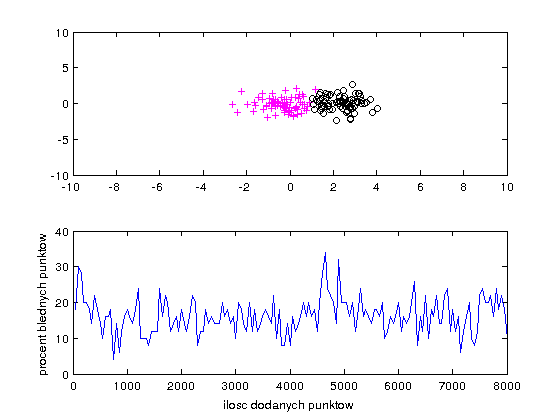
\includegraphics[width=\textwidth]{test3_h1_16_32.png}
    \caption{h = 1}
  \end{subfigure}
  
   \begin{subfigure}[b]{0.5\textwidth}
    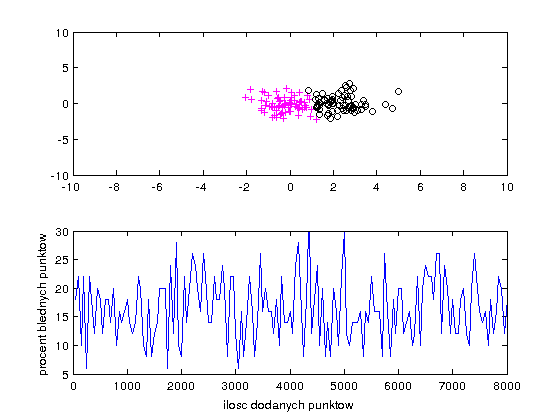
\includegraphics[width=\textwidth]{test3_h10_16_52.png}
    \caption{h = 10}
  \end{subfigure}
  \hfill
    \begin{subfigure}[b]{0.5\textwidth}
    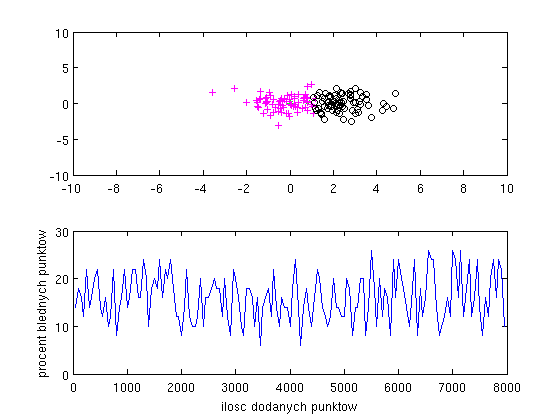
\includegraphics[width=\textwidth]{test3_h100_16_70.png}
    \caption{h = 100}
  \end{subfigure}
  
  
  
  \caption{Test zestawu 1 dla różnych h}
  \label{test_h3}
  
\end{figure}



\begin{table}[H]
\centering
\begin{tabular}{|c|c|}
\hline
spread & błąd \\
\hline
0,001 & 50\%  \\
\hline
0,01 & 29\%  \\
\hline
0,1 & 18\%  \\
\hline
1 & 16\%  \\
\hline
10 & 17\%  \\
\hline
100 & 16\%  \\
\hline
\end{tabular}
\caption{Zestawienie wyników testów dla stałych wartości spread dla zestawu 1.}
\label{h_table3}
\end{table}

Wyniki dla zestawu drugiego przedstawia rysunek \ref{test_h4} oraz tabela \ref{h_table4}.

\begin{figure}[H]

   \begin{subfigure}[b]{0.5\textwidth}
    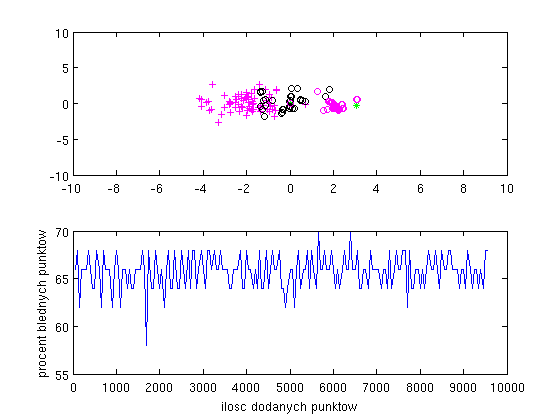
\includegraphics[width=\textwidth]{test4_h0_001_66_00.png}
    \caption{h = 0,001}
  \end{subfigure}
  \hfill
  \begin{subfigure}[b]{0.5\textwidth}
    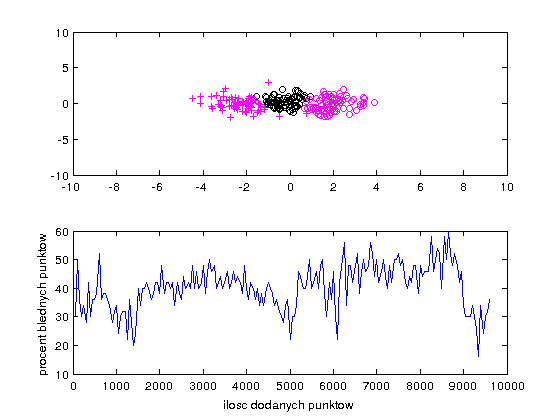
\includegraphics[width=\textwidth]{test4_h0_01_40_42.png}
    \caption{h = 0,01}
  \end{subfigure}
  
   \begin{subfigure}[b]{0.5\textwidth}
    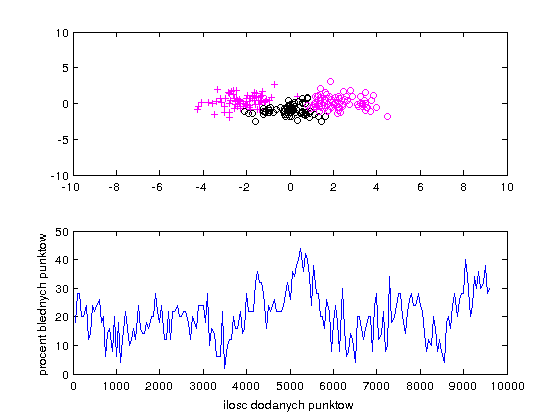
\includegraphics[width=\textwidth]{test4_h0_1_20_63.png}
    \caption{h = 0,1}
  \end{subfigure}
  \hfill
  \begin{subfigure}[b]{0.5\textwidth}
    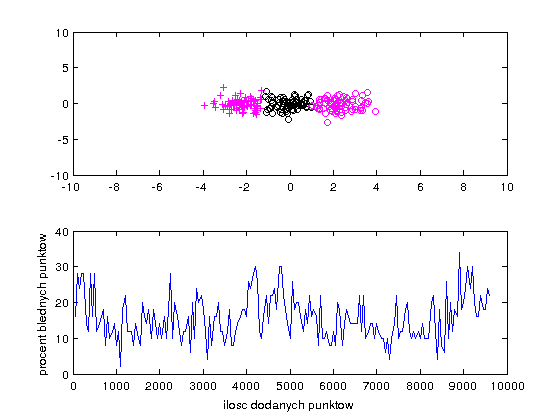
\includegraphics[width=\textwidth]{test4_h1_15_66.png}
    \caption{h = 1}
  \end{subfigure}
  
  \begin{subfigure}[b]{0.5\textwidth}
    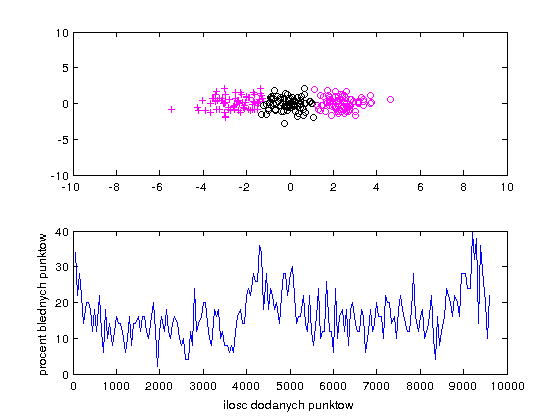
\includegraphics[width=\textwidth]{test4_h10_16_60.png}
    \caption{h = 10}
  \end{subfigure}
  \hfill
  \begin{subfigure}[b]{0.5\textwidth}
    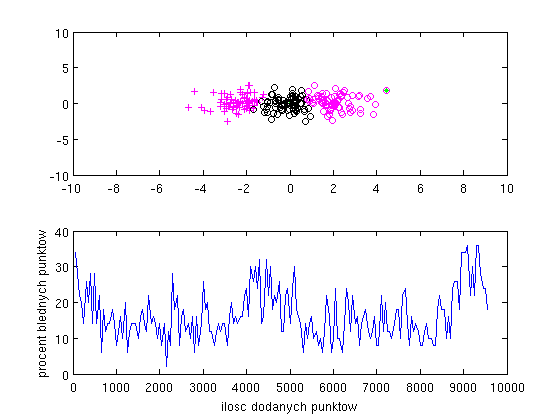
\includegraphics[width=\textwidth]{test4_h100_16_60.png}
    \caption{h = 100}
  \end{subfigure}
  
  
  \caption{Test zestawu 2 dla różnych h}
  \label{test_h4}
  
\end{figure}



\begin{table}[H]
\centering
\begin{tabular}{|c|c|}
\hline
spread & błąd \\
\hline
0,001 & 66\%  \\
\hline
0,01 & 40\%  \\
\hline
0,1 & 20\%  \\
\hline
1 & 15\%  \\
\hline
10 & 17\%  \\
\hline
100 & 17\%  \\
\hline
\end{tabular}
\caption{Zestawienie wyników testów dla stałych wartości spread dla zestawu 2.}
\label{h_table4}
\end{table}

\section{Wnioski}
Spoglądając na wyniki dla różnych wartości spread można zauważyć ciekawe zjawiska. Dla bardzo małej wartości błąd utrzymywał się na poziomie 50\%. Wynika to z faktu, że sieć rozpoznawała tylko punkty nauczone w poprzedniej iteracji, gdyż zasięg funkcji bazowej był praktycznie zerowy. W miarę zwiększania parametru wygładzania, błąd się zmniejszał, by osiągnąć minimalną wartość dla spread równego 1. Kiedy wartość była dalej zwiększana, błąd rósł, ale tylko dla metody oknowej, ponieważ zasięg funkcji bazowych był tak duży, że nawet punkty wyuczone w poprzedniej iteracji były błędnie klasyfikowane. W metodzie priorytetowej ustawienie wartości spread nawet na bardzo duże wartości nie powodowało znaczącego pogorszenia wyniku. Było to spowodowane faktem, że metoda ta opierała się na priorytetach, więc nawet dla dużych wartości parametru wygładzania punkty leżące bliżej skupiska danej klasy miały większy priorytet. W czasie trwania symulacji nie zauważono znaczącego wpływu przemieszczania się punktów drugiej klasy w pierwszym zestawie na błędne sklasyfikowane punkty. W drugim zestawie dla obydwu metod wyło widać wyraźny wzrost błędu w momencie, kiedy krążąca klasa przechodziła przez środek układu współrzędnych, gdzie "było" wąsko.  Należy przy tym zwrócić uwagę, że względny wzrost był dużo mniejszy przy metodzie priorytetowej. Działo się tak, ponieważ ta metoda wybierała tylko te punkty, co do których ma największą pewność -  punkty leżące w środkowej części klasy nie zmieszane z dwoma pozostałymi.  

Symulacja z automatycznym liczeniem współczynnika wygładzania działa podobnie jak dla optymalnie wybranego parametru h. Współczynnik oscylował w okolicach wartości 1. 

Podsumowując, wiele zależy od danych, które otrzymujemy. Jeśli obie klasy były by wystarczająco oddalone od siebie, poziom błędów byłby dużo mniejszy. Na stworzonym przykładzie poziom błędów nie zmieniał się znacznie w czasie, co dobrze świadczyło o adaptacji sieci neuronowe. W kwestii współczynnika spread można albo ustawić metodami prób i błędów wartość na sztywno i liczyć, że z czasem wartość tego parametru będzie nadal aktualna lub użyć funkcji obliczającej automatycznie ten parametr i mieć pewność, że jakość działania sieci będzie bardziej adaptatywna. 

\section{Kod}
Plik \textbf{method1\_example1.m} generuje symulację dla metody kolejkowej i zestawu 1. \\
Plik \textbf{method1\_example1\_dynamic\_spread.m} generuje symulację dla metody kolejkowej i zestawu 1 z automatycznym h. \\
Plik \textbf{method1\_example2.m} generuje symulację dla metody kolejkowej i zestawu 2. \\
Plik \textbf{method1\_example2\_dynamic\_spread.m} generuje symulację dla metody kolejkowej i zestawu 2 z automatycznym h. \\
Plik \textbf{method2\_example1.m} generuje symulację dla metody priorytetowej i zestawu 1. \\
Plik \textbf{method2\_example2.m} generuje symulację dla metody priorytetowej i zestawu 2. \\
\\
W metodzie priorytetowej współczynnik spread ustawia się w pliku \textbf{considerPoint.m} zmienną sigma




\end{document}